\documentclass{beamer}

\usepackage{pgfplots}
\usepackage{tkz-fct}
\usetkzobj{all}

\begin{document}

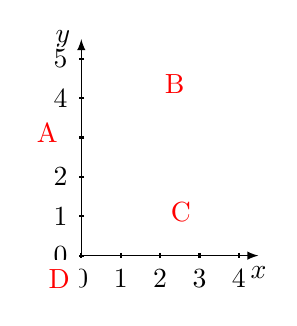
\begin{tikzpicture}[scale=.5]
\tkzInit[xmax=4,ystep=1,ymax=5]
\tkzAxeXY

\tkzFct[color=red, thick,domain=0:2]{\x*2}
\tkzFct[color=red, thick,domain=0:2]{\x*(-0.5)+2.5}
\tkzFct[color=red, thick,domain=0:2]{\x*(0.75)+2.5}
\tkzFct[color=red, thick,domain=0:2]{\x*(0.75)}
\tkzFct[color=red, thick,domain=1.97:1.987]{\x*150)-1.96*150}
\node[above right=15pt of {(1,3)}, outer sep=2pt,fill=white] {B};
\node[above right=10pt of {(-2,2)}, outer sep=2pt,fill=white] {A};
\node[above right=10pt of {(1.4,0)}, outer sep=2pt,fill=white] {C};
\node[above right=10pt of {(-1.7,-1.7)}, outer sep=2pt,fill=white] {D};

\end{tikzpicture}
\begin{tikzpicture}[scale=.5]

\end{tikzpicture}  
\end{document}